\section{Software}

The submarine's software is aware of the competition objectives, and performs computer vision to
command the submarine to move through the embedded system.
The software is organized so that it is easy to test the core vision and control systems with different
sources of video input and to command the submarine or the simulator to move.
The software also includes a graphical simulator that we can use to test our vision and control algorithms.

\subsection{Software Organization}
\label{gui}


\begin{figure}
\begin{center}
 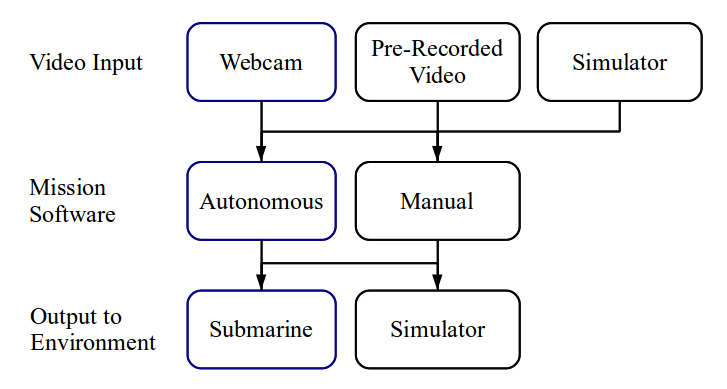
\includegraphics[height=1.9in]{fig/modules.png}
\caption{Software module organization.}\label{modules}
\end{center}
\end{figure}


\begin{figure}
\begin{center}
 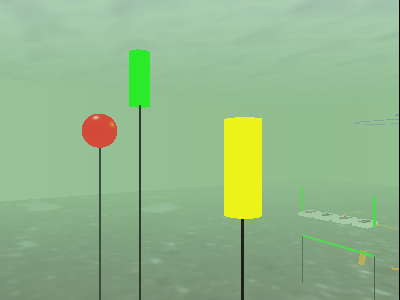
\includegraphics[height=1.9in]{fig/sim.png}
\caption{Example image from the simulator showing pipe segments and the buoys
         in turbid water.}\label{sim}
\end{center}
\end{figure}

The software is broken down into 3
components (Figure~\ref{modules}): (i) the video input;
(ii) the mission software gives physical commands to move the sub;
and (iii) the environment that reacts to the physical commands.
The video input can come from the submarine's webcams, pre-recorded video,
or the simulator (Figure~\ref{sim}). The mission software can be the autonomous
algorithms that drive the submarine or a manually controlled user interface.
The environment that reacts to physical commands can be the submarine or the
simulator. The different permutations to hook up the software components
solely created to test and debug the vision
algorithms when AquaTux is not functioning autonomously.
These software interfaces help ensure the software to test the submarine
resembles the autonomous functionality as much as possible.
The manual user interface allows us to act as a passive observer,
constantly requesting the state of the vehicle,
or as a controller sending commands to the AUV.

\subsection{Simulator}
The simulator is a piece of software written in C++ using the OpenGL library. Its purpose is to simulate the competition grounds so the software and vision algorithms can be tested with greater ease. The simulator was extremely useful, as using a pool is both expensive and time consuming.

The simulator contains a physical model of each obstacle in the competition,  as well as a method to track the locations of the two cameras on the sub. OpenGL calls are then used to draw the images that would be seen by the cameras, which are then extracted to the image processing algorithms (Figure~\ref{sim} shows an image that would be seen by the forward camera).
The simulator can accept commands to move the camera viewpoint, so that we can properly simulate video feedback when the submarine is commanded to move.

\subsection{Software Control}
Our control algorithms are run the submarine runs autonomously. The entire mission is broken down into tasks, such as the gate or buoy task,
which are implemented in separate modules. The control code queries the vision system for circles, lines or rectangles, and translates the
vision result into a movement command. While the submarine is reacting to a movement command, the video input is ignored to prevent
overshooting or oscillating the target.
Each control task can be tested separately.

\section{Vision}
The machine vision system is defined as all software and hardware which converts images (the input to the system) into numerical data (the output). This data refers primarily to the existence, position, orientation, and color of various objects in the image, such as the starting gate or a colored buoy. This information is handed off to the rest of the software, which acts on it to determine the correct course of action for the submarine. Because the internal representation of an image is simply a large matrix of numbers, the vision system's job can be thought of as filtering this large volume of mostly extraneous data to a few pieces of useful data, which the control system can then analyze.

\subsection{Vision Hardware}
The hardware for the vision subsystem consists of two cameras and a small netbook. Both cameras are Logitech Webcam 9000 Pro webcams, one of which points forward, and the other of which points down. These cameras were chosen for their price (about \$50 each) and the availability ofLinux driver support. While the cameras are not specifically designed for underwater or low light conditions, they have worked quite well in our pool testing. The netbook used is an HP <Model Number>. This model was chosen for its small size and low cost.

\subsection{Vision Software}
All of our image processing code is written in C++, using the OpenCV library. A large number of algorithms were tried and discarded during the development of our final flow.  Due to the scope of this document only the final algorithms used will be described.

The image processing flow can be broken up into three distinct parts: image segmentation (separating a 3-channel image into 1-channel pieces based primarily on color), object recognition (classification of each segment as background or target) and property calculation (deriving the object's properties such as location or color). The algorithm used for each step is distinct and will be discussed below.

Image segmentation is performed using OpenCV's implementation of the Watershed algorithm. The algorithm works iteratively from a collection of segmented pixels (seeds) and at each step associates the most similar pixel adjacent to a segmented pixel with that segment. It returns a grayscale image, with different gray levels corresponding to different segments. Each seed pixel has a value associated and two seeds of the same value will contribute to a single segment.

The performance of the Watershed algorithm is heavily dependent on the quality of the seeding. Optimally we want at least one seed for each different object in the image and at least one seed for the background. A single object should not have two different valued seeds, as this will cause two segments to emerge. To seed the algorithm, we take a random sample of pixels from the source image, and run K-Means clustering to cluster the samples based on color similarity. The results of the clustering is a minimum collection of pixels which are representative of the color space of the image. The clustering results used to assign values to the seeds - similarly colored seeds will get the same values (Figures~\ref{seed} and \ref{segment}).

\begin{figure}
\begin{center}
 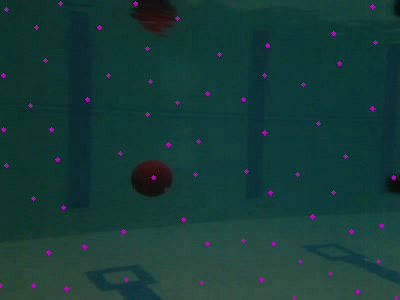
\includegraphics[height=1.9in]{fig/seed_image.jpg}
\caption{Example image at a test pool, with seed locations overlayed.}\label{seed}
\end{center}
\end{figure}


\begin{figure}
\begin{center}
 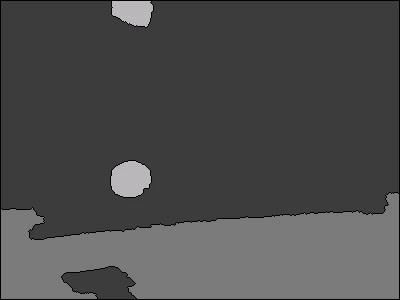
\includegraphics[height=1.9in]{fig/segmented_image.jpg}
\caption{The test image segmented.}\label{segment}
\end{center}
\end{figure}

Object recognition is made simple due to the fact that only circles and rectangles need to be recognized for the tasks we are aiming to do. OpenCV can find the minimum enclosing circle and (rotated) box for any segment, and a simple comparison of area, perimeter, and various symmetry properties can be performed to check if the segment is similar to its enclosing shape. For example, a the minimum enclosing circle of a non-circular segment will leave large amounts of blank space, and will therefore have a very different area compared to the segment.

Property calculation is done on a target-by-target basis. For most targets (the buoy, for example), it is  sufficient to know the position and characteristic dimension in pixel space. We can then use these numbers, along with the camera's field-of-view and the physical length to calculate the position and range of the object in real space. For the pipes at the bottom of the pool, the position angle is also needed. All of the pixle properties are easily extracted from the enclosing shape derived by OpenCV. To identify an object's color, we convert the BGR color of the object into HSV, which is more robust against changes in brightness, and use the resulting hue value to determine the color of the object.

Finally, in order for the vision code to return stable results and be robust against noise, we store the objects identified in the current frame begin processed as well as a number of frames prior. We use this to average and filter the numerical information from multiple frames. This allows us some room for error - a single frame with poor segmentation or a stray object will not destroy the system's performance.
